\chapter{Preliminaries}
\label{chap:introduction}

In today's information society, extraction of knowledge is becoming a very
important task for many people. We live in an age of knowledge revolution.
Peter Drucker~\cite{Drucker}, an influential management expert, writes ``From now on, the key is knowledge. The world is not becoming labor intensive, not material intensive, not energy intensive, but knowledge  intensive''.
This knowledge revolution is based in an economic 
change from adding value by producing things which is, ultimately 
limited, to adding value by creating and using knowledge which can 
grow indefinitely.

The digital universe in 2007 was estimated in~\cite{IDC} to be 281 exabytes
or 281 billion gigabytes, and by 2011, the digital universe will be 
10 times the size it was 5 years before. The amount of information created, 
or captured %, or replicated 
exceeded available storage for the first time in
2007. 

To deal with these huge amount of data in a responsible way,
green computing is becoming a necessity. {\em Green computing} 
is the study and practice of using computing resources efficiently.
A main approach to green computing is based on algorithmic efficiency.
The amount of computer resources required for any given computing function
depends on the efficiency of the algorithms used. As the cost of hardware
has declined relative to the cost of energy, the energy efficiency and 
environmental impact of computing systems and programs 
are receiving increased attention.


\section{MOA Stream Mining }

A largely untested hypothesis of modern society is that it is important to record data as it may contain valuable information. This occurs in almost all facets of life from supermarket checkouts to the movements of cows in a paddock. To support the hypothesis, engineers and scientists have produced a raft of ingenious schemes and devices from loyalty programs to RFID tags. Little thought however, has gone into how this {\em quantity} of data might be analyzed. 

{\em Machine learning}, the field for finding ways to automatically extract information from data, was once considered the solution to this problem. Historically it has concentrated on learning from small numbers of examples, because only limited amounts of data were available when the field emerged. Some very sophisticated algorithms have resulted from the research that can learn highly accurate models from limited training examples. It is commonly assumed that the entire set of training data can be stored in working memory.

More recently the need to process larger amounts of data has motivated the field of {\em data mining}. Ways are investigated to reduce the computation time and memory needed to process large but static data sets. If the data cannot fit into memory, it may be necessary to sample a smaller training set. Alternatively, algorithms may resort to temporary external storage, or only process subsets of data at a time. Commonly the goal is to create a learning process that is linear in the number of examples. The essential learning procedure is treated like a scaled up version of classic machine learning, where learning is considered a single, possibly expensive, operation---a set of training examples are processed to output a final static model.

The data mining approach may allow larger data sets to be handled, but it still does not address the problem of a {\em continuous} supply of data. Typically, a model that was previously induced cannot be updated when new information arrives. Instead, the entire training process must be repeated with the new examples included. There are situations where this limitation is undesirable and is likely to be inefficient.

The {\em data stream} paradigm has recently emerged in response to the continuous data problem. Algorithms written for data streams can naturally cope with data sizes many times greater than memory, and can extend to challenging real-time applications not previously tackled by machine learning or data mining. The core assumption of data stream processing is that training examples can be briefly inspected a single time only, that is, they arrive in a high speed stream, then must be discarded to make room for subsequent examples. The algorithm processing the stream has no control over the order of the examples seen, and must update its model incrementally as each example is inspected. An additional desirable property, the so-called {\em anytime} property, requires that the model is ready to be applied at any point between training examples.

\BEGINOMIT
The {\em Hoeffding tree} induction method, a method for producing {\em decision tree} models, represents one of the best known algorithms for classifying streams of examples. Improvements to it are the focus of this \thesis. As the method is already state-of-the-art, it is not expected that massive gains will be possible, but rather smaller incremental improvements that are beneficial nonetheless. To measure improvements to this algorithm, an evaluation framework is developed to provide useful insight about classification performance. This fosters algorithm development that results in measurably improved performance.
\ENDOMIT

Studying purely theoretical advantages of algorithms is certainly useful and enables new developments, but the demands of data streams require this to be followed up with empirical evidence of performance. Claiming that an algorithm is suitable for data stream scenarios implies that it possesses the necessary practical capabilities. Doubts remain if these claims cannot be backed by reasonable empirical evidence.

%A central argument of this \thesis is that D
Data stream classification algorithms require appropriate and complete evaluation practices. The evaluation should allow users to be sure that particular problems can be handled, to quantify improvements to algorithms, and to determine which algorithms are most suitable for their problem. \textbf{MOA} is suggested with these needs in mind.

Measuring data stream classification performance is a three dimensional problem involving processing speed, memory and accuracy. It is not possible to enforce and simultaneously measure all three at the same time so in %a new framework as
 \textbf{MOA} %this \thesis argues that 
it is necessary to fix the memory size and then record the other two. Various memory sizes can be associated with data stream application scenarios so that basic questions can be asked about expected performance of algorithms in a given application scenario. \textbf{MOA} is developed to provide useful insight about classification performance.


\section{Assumptions}

%This \thesis 
\textbf{MOA} is concerned with the problem of {\em classification}, perhaps the most commonly researched machine learning task. The goal of classification is to produce a model that can predict the class of unlabeled examples, by training on examples whose label, or {\em class}, is supplied. To clarify the problem setting being addressed, several assumptions are made about the typical learning scenario: 
\begin{enumerate}
\item The data is assumed to have a small and fixed number of columns, or {\em attributes}/{\em features}---several hundred at the most. 
\item The number of rows, or {\em examples}, is very large---millions of examples at the smaller scale. 
In fact, algorithms should have the potential to process an infinite amount of data, meaning that they will not exceed memory limits or otherwise fail no matter how many training examples are processed.
\item The data has a limited number of possible class labels, typically less than ten.
\item The amount of memory available to a learning algorithm depends on the application. The size of the training data will be considerably larger than the available memory.
\item There should be a small upper bound on the time allowed to train or classify an example. This permits algorithms to scale linearly with the number of examples, so users can process $N$ times more than an existing amount simply by waiting $N$ times longer than they already have. 
\item Stream concepts are assumed to be stationary or evolving. % in the first part, that is, the problem of {\em concept drift} is not directly addressed until the second part. 
Concept drift occurs when the underlying concept defining the target being learned begins to shift over time. %The solutions explored here could be extended to handle concept drift, but this is reserved for future work.
\end{enumerate}

The first three points emphasize that the aim is to scale with the number of examples. Data sources that are large in other dimensions, such as numbers of attributes or possible labels are not the intended problem domain. Points 4 and 5 outline what is needed from a solution. Regarding point 6, some researchers argue that addressing concept drift is one of the most crucial issues in processing data streams. %For this \thesis it is believed more important that the other requirements are met first, otherwise a solution will not be satisfactory when demands are too high regardless of whether concept drift is addressed.

\section{Requirements} 

The conventional machine learning setting, referred to in this \thesis as the {\em batch} setting, operates assuming that the training data is available as a whole set---any example can be retrieved as needed for little cost. An alternative is to treat the training data as a \emph{stream}, a potentially endless flow of data that arrives in an order that cannot be controlled.
Note that an algorithm capable of learning from a stream is, by definition, a data mining algorithm.

Placing classification in a data stream setting offers several advantages. Not only is the limiting assumption of early machine learning techniques addressed, but other applications even more demanding than mining of large databases can be attempted. An example of such an application is the monitoring of high-speed network traffic, where the unending flow of data is too overwhelming to consider storing and revisiting.

A classification algorithm must meet several requirements in order to work with the assumptions and be suitable for learning from data streams. The requirements, numbered 1 through 4, are detailed below.


\subsection*{Requirement 1: Process an example at a time, and inspect it only once (at most)}

The key characteristic of a data stream is that data `flows' by one example after another. There is no allowance for \emph{random access} of the data being supplied. Each example must be accepted as it arrives in the order that it arrives. Once inspected or ignored, an example is discarded with no ability to retrieve it again.

Although this requirement exists on the input to an algorithm, there is no rule preventing an algorithm from remembering examples internally in the short term. An example of this may be the algorithm storing up a \emph{batch} of examples for use by a conventional learning scheme. While the algorithm is free to operate in this manner, it will have to discard stored examples at some point if it is to adhere to requirement 2.

The inspect-once rule may only be relaxed in cases where it is practical to re-send the entire stream, equivalent to multiple scans over a database. In this case an algorithm may be given a chance during subsequent passes to refine the model it has learned. However, an algorithm that requires any more than a single pass to operate is not flexible enough for universal applicability to data streams.

\subsection*{Requirement 2: Use a limited amount of memory}

The main motivation for employing the data stream model is that it allows processing of data that is many times larger than available working memory. The danger with processing such large amounts of data is that memory is easily exhausted if there is no intentional limit set on its use.

Memory used by an algorithm can be divided into two categories: memory used to store running statistics, and memory used to store the current model. For the most memory-efficient algorithm they will be one and the same, that is, the running statistics directly constitute the model used for prediction.

This memory restriction is a physical restriction that can only be relaxed if external storage is used, temporary files for example. Any such work-around needs to be done with consideration of requirement 3.

\subsection*{Requirement 3: Work in a limited amount of time}

For an algorithm to scale comfortably to any number of examples, its runtime complexity must be linear in the number of examples. This can be achieved in the data stream setting if there is a constant, preferably small, upper bound on the amount of processing per example.

Furthermore, if an algorithm is to be capable of working in \emph{real-time}, it must process the examples as fast if not faster than they arrive. Failure to do so inevitably means loss of data.

Absolute timing is not as critical in less demanding applications, such as when the algorithm is being used to classify a large but persistent data source. However, the slower the algorithm is, the less value it will be for users who require results within a reasonable amount of time.

\subsection*{Requirement 4: Be ready to predict at any point}

An ideal algorithm should be capable of producing the best model it can from the data it has observed after seeing any number of examples. In practice it is likely that there will be periods where the model stays constant, such as when a batch based algorithm is storing up the next batch.

The process of generating the model should be as efficient as possible, the best case being that no translation is necessary. That is, the final model is directly manipulated in memory by the algorithm as it processes examples, rather than having to recompute the model based on running statistics. 

\subsection*{The data stream classification cycle}

\begin{figure}
\centering
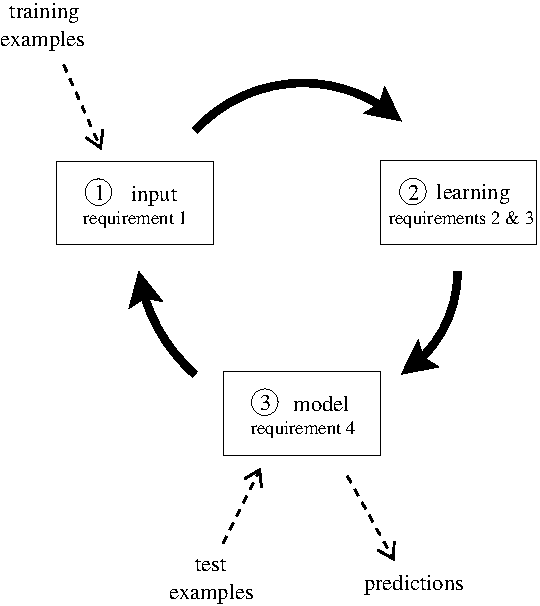
\includegraphics{figures/ds_cycle}
\caption{The data stream classification cycle.}
\label{fig:ds_cycle}
\end{figure}

Figure~\ref{fig:ds_cycle} illustrates the typical use of a data stream classification algorithm, and how the requirements fit in. The general model of data stream classification follows these three steps in a repeating cycle:

\begin{enumerate}

\item The algorithm is passed the next available example from the stream (requirement 1).

\item The algorithm processes the example, updating its data structures. It does so without exceeding the memory bounds set on it (requirement 2), and as quickly as possible (requirement 3).

\item The algorithm is ready to accept the next example. On request it is able to supply a model that can be used to predict the class of unseen examples (requirement 4).

\end{enumerate}

\section{Mining Strategies} 

The task of modifying machine learning algorithms to handle large data sets is known as {\em scaling up}~\cite{ml_scaleup}.
Analogous to approaches used in data mining, there are two general strategies for taking machine learning concepts and applying them to data streams. The \emph{wrapper} approach aims at maximum reuse of existing schemes, whereas \emph{adaptation} looks for new methods tailored to the data stream setting.

Using a wrapper approach means that examples must in some way be collected into a batch so that a traditional batch learner can be used to induce a model. The models must then be chosen and combined in some way to form predictions. The difficulties of this approach include determining appropriate training set sizes, and also that training times will be out of the control of a wrapper algorithm, other than the indirect influence of adjusting the training set size. When wrapping around complex batch learners, training sets that are too large could stall the learning process and prevent the stream from being processed at an acceptable speed. Training sets that are too small will induce models that are poor at generalizing to new examples. Memory management of a wrapper scheme can only be conducted on a per-model basis, where memory can be freed by forgetting some of the models that were previously induced. Examples of wrapper approaches from the literature include Wang et al.~\cite{cdensemble}, Street and Kim~\cite{sea} and Chu and Zaniolo~\cite{fastlightboost}. 

Purposefully adapted algorithms designed specifically for data stream problems offer several advantages over wrapper schemes. They can exert greater control over processing times per example, and can conduct memory management at a finer-grained level.
Common varieties of machine learning approaches to classification fall into several general classes. These classes of method are discussed below, along with their potential for adaptation to data streams:


\begin{description}
\item[decision trees] This class of method is the main focus of the \thesis. Chapter~\ref{chap:hoeffdingtrees} studies a successful adaptation of decision trees to data streams~\cite{vfdt} and outlines the motivation for this choice.
\item[rules] Rules are somewhat similar to decision trees, as a decision tree can be decomposed into a set of rules, although the structure of a rule set can be more flexible than the hierarchy of a tree. Rules have an advantage that each rule is a disjoint component of the model that can be evaluated in isolation and removed from the model without major disruption, compared to the cost of restructuring decision trees. However, rules may be less efficient to process than decision trees, which can guarantee a single decision path per example. Ferrer-Troyano et al.~\cite{scallop, dsrules} have developed methods for inducing rule sets directly from streams.
\item[lazy/nearest neighbour] This class of method is described as {\em lazy} because in the batch learning setting no work is done during training, but all of the effort in classifying examples is delayed until predictions are required. The typical {\em nearest neighbour} approach will look for examples in the training set that are most similar to the example being classified, as the class labels of these examples are expected to be a reasonable indicator of the unknown class. The challenge with adapting these methods to the data stream setting is that training can not afford to be lazy, because it is not possible to store the entire training set. Instead the examples that are remembered must be managed so that they fit into limited memory. An intuitive solution to this problem involves finding a way to merge new examples with the closest ones already in memory, the main question being what merging process will perform best. Another issue is that searching for the nearest neighbours is costly. This cost may be reduced by using efficient data structures designed to reduce search times. Nearest neighbour based methods are a popular research topic for data stream classification. Examples of systems include~\cite{anncad, lwclass, ds-knn, ds-instancebased}.
\item[support vector machines/neural networks] Both of these methods are related and of similar power, although {\em support vector machines}~\cite{svm} are induced via an alternate training method and are a hot research topic due to their flexibility in allowing various {\em kernels} to offer tailored solutions.
Memory management for support vector machines could be based on limiting the number of support vectors being induced. Incremental training of support vector machines has been explored previously, for example~\cite{incrsvm}.
Neural networks are relatively straightforward to train on a data stream. A real world application using neural networks is given by Gama and Rodrigues~\cite{gama_ann}. The typical procedure assumes a fixed network, so there is no memory management problem. It is straightforward to use the typical {\em backpropagation} training method on a stream of examples, rather than repeatedly scanning a fixed training set as required in the batch setting.
\item[Bayesian methods] These methods are based around {\em Bayes' theorem} and compute probabilities in order to perform {\em Bayesian inference}. The simplest Bayesian
method, Naive Bayes, is described in Section~\ref{sec:nbleaf}, and is a special case of algorithm that needs no adaptation to data streams. This is because it is straightforward to train incrementally and does not add structure to the model, so that memory usage is small and bounded. A single Naive Bayes model will generally not be as accurate as more complex models. The more general case of {\em Bayesian networks} is also suited to the data stream setting, at least when the structure of the network is known. Learning a suitable structure for the network is a more difficult problem. Hulten and Domingos~\cite{mineabitrarydb} describe a method of learning Bayesian networks from data streams using Hoeffding bounds. Bouckaert~\cite{remcobayesstream} also presents a solution.
\item[meta/ensemble methods] These methods wrap around other existing methods, typically building up an {\em ensemble} of models. Examples of this include~\cite{ozabagboost, anncad}. This is the other major class of algorithm studied in-depth by this \thesis, beginning in Chapter~\ref{chap:improvebackground}.
\end{description}

Gaber et al.~\cite{dssurvey} survey the field of data stream classification algorithms and list those that they believe are major contributions. Most of these have already been covered: Domingos and Hulten's {\em VFDT}~\cite{vfdt}, the decision tree algorithm studied in-depth by this \thesis; {\em ensemble-based classification} by Wang et al.~\cite{cdensemble} that has been mentioned as a wrapper approach; {\em SCALLOP}, a rule-based learner that is the earlier work of Ferrer-Troyano et al.~\cite{scallop}; {\em ANNCAD}, which is a nearest neighbour method developed by Law and Zaniolo~\cite{anncad} that operates using {\em Haar wavelet} transformation of data and small classifier ensembles; and {\em LWClass} proposed by Gaber et al.~\cite{lwclass}, another nearest neighbour based technique, that actively adapts to fluctuating time and space demands by varying a distance threshold. The other methods in their survey that have not yet been mentioned include {\em on demand classification}. This method by Aggarwal et al.~\cite{ondemand} performs dynamic collection of training examples into supervised {\em micro-clusters}. From these clusters, a nearest neighbour type classification is performed, where the goal is to quickly adapt to concept drift. The final method included in the survey is known as an {\em online information network} ({\em OLIN}) proposed by Last~\cite{olin}. This method has a strong focus on concept drift, and uses a {\em fuzzy} technique to construct a model similar to decision trees, where the frequency of model building and training window size is adjusted to reduce error as concepts evolve.

\BEGINOMIT
Of the broad classes of algorithm, there are no existing benchmarks to determine which class is superior to any other at classifying data streams. Decision trees were chosen because they are a classic area of research, and there is existing evidence to suggest that they are an effective method for data stream classification.


\section{Thesis Structure}

The chapters that follow build the \thesis in logical sequence:

Chapter~\ref{chap:experimentalsetting} reviews the common methodologies in practice for evaluating data stream algorithms. After considering the desirable attributes of a comprehensive evaluation strategy a final framework is proposed. The framework includes simulation of three environments by varying memory demands, and a set of synthetic data generators in preparation for evaluation of  learning algorithms in the \thesis.

Chapter~\ref{chap:hoeffdingtrees} introduces the basic decision tree learning algorithm that operates on data streams by relying on Hoeffding bounds to decide when sufficient information has been seen to justify tree expansion. Many aspects of the basic algorithm are explored.

Chapter~\ref{chap:numericatts} sets out to resolve the issue of how Hoeffding trees should handle continuous numeric attributes. Potential approaches are surveyed, and then candidates are tested using the evaluation framework from Chapter~\ref{chap:experimentalsetting} in an experiment to determine which strategy performs best.

Chapter~\ref{chap:predstrat} conducts a study of prediction methods, using the evaluation framework from Chapter~\ref{chap:experimentalsetting} to produce empirical evidence in support of a newly suggested method. This hybrid approach adaptively combines the strengths of two previous methods.

Chapter~\ref{chap:improvebackground} surveys common methods for improving accuracy in the batch setting via ensembles of models. Possibilities for transferring these methods to data streams are explored, along with the theoretical implications of combining increasing numbers of models when memory is limited. Algorithms are elaborated, including a novel method of inducing {\em option trees}---a generalized representation of decision trees offering the benefits of ensembles in a single and potentially more memory-efficient structure.

Chapter~\ref{chap:improvecompare} experimentally compares the main algorithms suggested in Chapter~\ref{chap:improvebackground} using the evaluation framework from Chapter~\ref{chap:experimentalsetting}. Some of the results on data stream problems are surprising, and some do not entirely match the expectations arising from generalizations in the batch setting, so a deeper analysis and discussion looks more closely at the issues.

Chapter~\ref{chap:conclusions} summarizes the findings and lists the contributions made. It concludes with a discussion of potential for future work.
\ENDOMIT

%\section{Evolving Stream Mining Strategies}

 Dealing with time-changing data requires %in turn 
strategies for detecting and quantifying change, forgetting stale examples, 
and for model revision. Fairly generic strategies exist for detecting
change and deciding when examples are no longer relevant. %Model revision
%strategies, on the other hand, are in most cases method-specific.
\BEGINOMIT
Most strategies for dealing with time change contain hardwired constants, 
or else require input parameters, concerning the expected speed or frequency 
of the change; some examples are {\em a priori} definitions of sliding window
lengths, values of decay or forgetting parameters, explicit bounds on maximum drift, etc. 
%\BEGINOMIT
These choices represent preconceptions 
on how fast or how often the data are going to evolve and, of course, they 
may be completely wrong. Even more, no fixed 
choice may be right, since the stream may experience any combination 
of abrupt changes, gradual ones, and long stationary periods. 
More in general, an approach based on fixed parameters will be caught in the following tradeoff: 
the user would like to use values of parameters that give more accurate statistics 
(hence, more precision) during periods of stability, but at the same time use the opposite values of
 parameters to %be able to 
quickly react to changes, when they occur. 
%\ENDOMIT

Many ad-hoc methods have been used to deal with drift, often tied to particular algorithms. 
%In Section~\ref{Sframework} %
\ENDOMIT
\BEGINOMIT
In this chapter we propose a more general approach based on using two primitive design 
elements: change detectors and estimators. 
The idea is to 
encapsulate all the statistical calculations having to do with detecting change and keeping
updated statistics from a stream an abstract data type that can then be used to replace, 
in a black-box way, the counters and accumulators that typically all machine learning
and data mining algorithms use to make their decisions, including when change has occurred. 

We believe that, compared to any previous approaches, our approach better isolates different
concerns when designing new data mining algorithms, therefore reducing design time,
increasing modularity, and facilitating analysis. Furthermore, since we crisply identify
the nuclear problem in dealing with drift, and use a well-optimized algorithmic solution to tackle it,
the resulting algorithms are more accurate, adaptive, and time- and memory-efficient than other
ad-hoc approaches. % starting from scratch. 
%We have given evidence for this superiority in \cite{bif-gav,Kbif-gav,KDD08}
%and we demonstrate this idea again here.

\subsection{Theoretical approaches}%Learning time-varying concepts}

The task of learning drifting or time-varying concepts has also been studied
 in computational learning theory. Learning a changing concept is infeasible,
 if no restrictions are imposed on the type of admissible concept changes,  
but drifting concepts are provably efficiently learnable (at least for certain 
concept classes), if the rate or the extent of drift is limited in particular ways. 

Helmbold and Long \cite{helmbold94tracking} assume a possibly permanent but slow concept 
drift and define the extent of drift as the probability that two subsequent 
concepts disagree on a randomly drawn example. Their results include an 
upper bound for the extend of drift maximally tolerable by any learner and 
algorithms that can learn concepts that do not drift more than a certain 
constant extent of drift. Furthermore they show that it is sufficient for a 
learner to see a fixed number of the most recent examples. Hence a window 
of a certain minimal fixed size allows to learn concepts for which the extent 
of drift is appropriately limited. 
While Helmbold and Long restrict the extend of drift, Kuh, Petsche, and 
Rivest~\cite{kuh} determine a maximal rate of drift that is acceptable by any learner, 
i. e. a maximally acceptable frequency of concept changes, which implies a 
lower bound for the size of a fixed window for a time-varying concept to be 
learnable, which is similar to the lower bound of Helmbold and Long. 

\ENDOMIT

%\section{Change Detection and Value Estimation}
%\label{SChange}
\section{Change Detection Strategies} 

The following different modes of change have been identified in the literature~\cite{tsymbal-problem,stanley03learning,WidmerKubat}:

\begin{itemize}
\item concept change
\begin{itemize}
\item concept drift
\item concept shift
\end{itemize}
\item distribution or sampling change
\end{itemize}

\textit{Concept} refers to the target variable, which the model is trying to predict.
\textit{Concept change} is the change of the underlying concept over time.
Concept drift describes a gradual change of the concept
and concept shift happens when a change between two concepts is more abrupt. 

\textit{Distribution change}, also known as sampling
change or shift or virtual concept drift , refers to the change in the data distribution.
Even if the concept remains the same, the change may often lead to revising the
current model as the model's error rate may no longer be acceptable with the
new data distribution.

Some authors, as Stanley~\cite{stanley03learning}, have suggested that from the practical point of view, it is not
essential to differentiate between concept change and sampling change since the
current model needs to be changed in both cases.
%We agree to some extent, and our methods will not be targeted to one particular type of change.
%Both cases of concept drift and concept shift abound in the
%real world. Since they have different characteristics, they may require different
%optimal prediction strategies.

%%%%%%%%%%%%%%%%%%%%%%%%%%%%%%%%%%%%%%%%%%%%%%%%%%%%%%%
%\subsection{Change Detection}

Change detection is not an easy task, since a fundamental
limitation exists~\cite{Gustaffson:2000}: the design of a change detector
is a compromise between detecting true changes and avoiding false
alarms. 
See~\cite{Gustaffson:2000,Baseville93} for more detailed surveys of change detection methods.

\subsubsection{The CUSUM Test}
\label{Sscusum}

The cumulative sum (CUSUM algorithm), %which was
 first proposed in \cite{Page54}, 
is a change detection algorithm that gives an alarm when the mean of the input data is significantly 
different from zero. The CUSUM input $\epsilon_t$ can be any filter residual, for instance 
the prediction error from a Kalman filter.

The CUSUM test is as follows:
$$g_0=0$$
$$g_t=\mbox{max }(0,g_{t-1}+ \epsilon_t -\upsilon)$$
$$\mbox{if } g_t>h \mbox{ then alarm and } g_t=0$$
%
The CUSUM test is memoryless, and its accuracy depends on the choice of parameters $\upsilon$ and $h$.

\subsubsection{The Geometric Moving Average Test}
\label{Ssgma}
The CUSUM test is a stopping rule. Other stopping rules exist. For example, the Geometric Moving Average (GMA) test,
first proposed in~\cite{Roberts}, is the following
$$g_0=0$$
$$g_t= \lambda g_{t-1}+ ( 1- \lambda) \epsilon_t$$
$$\mbox{if } g_t>h \mbox{ then alarm and } g_t=0$$
The forgetting factor $\lambda$ is used to give more or less weight to the last data arrived.
The treshold $h$ is used to tune the sensitivity and false alarm rate %performance 
of the detector.


\subsubsection{Statistical Tests}
\label{Ssstatic}

CUSUM and GMA are methods for dealing with numeric sequences. For more complex populations,
we need to use other methods.
There exist some statistical tests that may be used to detect change.
A statistical test is a procedure for deciding whether a hypothesis 
about a quantitative feature of a population is true or false. We test 
an hypothesis of this sort by drawing a random sample from the population
 in question and calculating an appropriate statistic on its items. 
If, in doing so, we obtain a value of the statistic that would occur
 rarely when the hypothesis is true, we would have reason to reject the hypothesis. 

To detect change, we need to compare two sources of data, and decide if
the hypothesis $H_0$ that they come from the same distribution is true. 
Let's suppose we have two estimates, $\hmu_0$ and $\hmu_1$ with variances
$\sigma_0^2$ and $\sigma_1^2$. If there is no change in the data, 
these estimates will be consistent. Otherwise, a hypothesis test will
reject $H_0$ and a change is detected. There are several ways to construct
such a hypothesis test. The simplest one is to study the difference

$$ \hmu_0 - \hmu_1 \in N(0, \sigma_0^2+ \sigma_1^2), \mbox{ under } H_0$$

or, to make a $\chi^ 2$ test

$$ \frac{(\hmu_0 - \hmu_1)^ 2}{\sigma_0^2+ \sigma_1^2} \in \chi^ 2(1), \mbox{ under } H_0$$

from which a standard hypothesis test can be formulated. 

For example, suppose we want to design a change detector using a statistical test
with a probability of false alarm of $5\%$, that is,

$$\Pr \left( \frac{|\hmu_0 - \hmu_1|}{\sqrt{\sigma_0^2+ \sigma_1^2}} > h \right) = 0.05$$

A table of the Gaussian distribution shows that $P( X< 1.96) = 0.975$, so the test becomes

$$\frac{(\hmu_0 - \hmu_1)^ 2}{{\sigma_0^2+ \sigma_1^2}} > 1.96$$
Note that this test uses the normality hypothesis. In Chapter~\ref{ch:adwin} we will propose a similar test with
theoretical guarantees. However, 
we could have used this test on the methods of Chapter~\ref{ch:adwin}.

The Kolmogorov-Smirnov test~\cite{Kanji} is another statistical test used to compare two populations.
Given samples %of size $n_1$ and $n_2$ 
from two populations, the cumulative distribution functions %$S_{n_1}(x)$ and $S_{n_2}(y)$ 
can be determined and plotted. Hence the maximum value of the difference between the plots can be found and compared with a critical value. If the
observed value exceeds the critical value, %the null hypothesis that the two population distributions are identical 
$H_0$ is rejected and a change is detected. It is not obvious how to implement the  Kolmogorov-Smirnov test dealing with data streams. Kifer et al.~\cite{kifer-detecting} propose a KS-structure to implement Kolmogorov-Smirnov and similar tests, on the data stream setting.

\subsubsection{Drift Detection Method}
\label{SsDDM}

The drift detection method (DDM) proposed by Gama et al.  \cite{Gama} controls the number of errors produced by
the learning model during prediction. %It uses a binomial distribution that 
%gives the general form of the probability for the random variable that represents the
It compares the statistics of two windows: the first one contains all the data, and the second one contains only the data from the beginning until the number of errors increases. This method does not store these windows in memory. It keeps only statistics and a window of recent data.% since a warning signal is detected.

The number of errors in a sample of $n$ examples is modelized by a binomial distribution. For each point $i$ in the sequence
that is being sampled, the error rate is the probability of misclassifying ($p_i$),
with standard deviation given by $s_i = \sqrt{p_i(1 - p_i)/i}$. It assumes (as can be argued e.g. in the
PAC learning model \cite{Mitchell}) that the error rate of the learning algorithm ($p_i$) will
decrease while the number of examples increases if the distribution of the examples is stationary. A significant increase in the error of the algorithm, suggests
that the class distribution is changing and, hence, the actual decision model is
supposed to be inappropriate. Thus, it stores the values of $p_i$ and $s_i$ when
$p_i+s_i$ reaches its minimum value during the process (obtaining $p_{pmin}$ and $s_{min}$),
and when the following conditions triggers:
\begin{itemize}
\item $p_i + s_i \geq p_{min} + 2 \cdot s_{min}$ for the warning level. Beyond this level, the examples are stored in anticipation of a possible change of context.

\item $p_i + s_i \geq p_{min} + 3 \cdot s_{min}$ for the drift level. Beyond this level the concept drift is supposed to be true, the model induced by the learning method is reset and a new model is learnt using the examples stored since the warning level triggered. The values for $p_{min}$ and $s_{min}$ are reset too.

\end{itemize}

This approach has a good behaviour of detecting abrupt changes and gradual
changes when the gradual change is not very slow, but it has difficulties when
the change is slowly gradual. In that case, the examples will be stored for long
time, the drift level can take too much time to trigger and the example memory
can be exceeded.

Baena-Garc\'{\i}a et al. proposed a new method EDDM in order to improve DDM. 
EDDM~\cite{EDDM} is shown to be better
than DDM for some data sets and worse for others. It is based on the 
estimated distribution of the distances between classification errors.
The window resize procedure is governed by the same heuristics.


%\subsection{Other change detection methods}
\label{Ssochange}


%\subsection{Estimation}
\subsubsection{Exponential Weighted Moving Average}
\label{Ssewma}

%The Estimator component
An Estimator is an algorithm that estimates the desired statistics on the input data, which
may change over time. %The algorithm may or may not use the data contained in the Memory. 
The simplest Estimator algorithm for the expected is the {\em linear estimator,}
which simply returns the average of the data items contained in the Memory. 
Other examples of run-time efficient estimators are 
Auto-Regressive, Auto Regressive Moving Average, and Kalman filters. 

An exponentially weighted moving average (EWMA) estimator is 
an algorithm that updates the estimation of a variable by combining the most 
recent measurement of the variable with the EWMA of all previous measurements:
$$ X_t=\alpha z_t + (1 -\alpha) X_{t-1} = X_{t-1} + \alpha (z_t -X_{t-1}) $$ 
where $X_t$ is the moving average, $z_t$ is the latest measurement, and $\alpha$
 is the weight given to the latest measurement (between 0 and 1). 
The idea is to produce an estimate that gives more weight to recent measurements, 
on the assumption that recent measurements are more likely to be relevant. 
Choosing an adequate $\alpha$ is a difficult problem, and it is not trivial.





